\documentclass[14pt, a4paper]{article}
\usepackage[x11names]{xcolor}
\usepackage[T1]{fontenc}
\usepackage{xltxtra}
\usepackage{graphicx}



\defaultfontfeatures{Mapping=tex-text}
\usepackage[top=1.2in,bottom=1.2in,left=1.2in,right=1in]{geometry}
\usepackage[boldfont,slantfont,CJKchecksingle]{xeCJK}
\xeCJKsetup{PunctStyle=hangmobanjiao}
\setlength{\parindent}{0cm}
\linespread{1.2}
\setlength{\parskip}{\baselineskip}

\XeTeXlinebreaklocale "zh"
\XeTeXlinebreakskip = 0pt plus 1pt minus 0.1pt

\usepackage[unicode=true,colorlinks,linkcolor=blue]{hyperref}
\setCJKmainfont[BoldFont=Source Han Sans CN, ItalicFont=Adobe Kaiti Std]{Source Han Serif CN}
\setmainfont{Noto Serif CJK SC}
\setmonofont{Noto Sans Mono CJK SC}
\setsansfont{Noto Sans CJK SC}

\usepackage{graphicx}  
\usepackage{longtable,booktabs}
\usepackage{pdflscape}

\renewcommand\contentsname{目录}
\renewcommand{\today}{\number\year 年 \number\month 月 \number\day 日} 


\usepackage{multicol}
\usepackage{indentfirst}
\usepackage{booktabs}
\usepackage{subfigure}
\usepackage{amsmath}
\setlength{\parindent}{2em}

\begin{document}
\title{\textbf{基于遗传算法的CMOS电路设计优化\\CMOS Circuit optimized by Genetic Algorithm}}
\author{广州大学\ 贺怡通}
\maketitle

\begin{abstract}
    \noindent
    \textbf{摘要: }在芯片设计中,调整各MOS管的参数至关重要。文中利用遗传算法实现了对电路多个性能指标同时优化。同时也可自定义的指标倾向以适应不同的电路设计环境。新方法在设计大规模集成电路的时候有明显的速度优势,降低了电路设计难度。\\
    \textbf{关键词: }CMOS, 遗传算法, 芯片设计 \\
    
    \noindent
    \textbf{Abstract: }Optimizing parameters is very important in IC Design. This paper presents a method to optimize the circuit indicators by genetic algorithm. At the same time, it can also adapt to different environments by setting targets. This new method has a speed advantage in IC Design and reduces the difficulty. \\
    \textbf{Key words:} CMOS, Genetic Algorithm, IC Design \\ \\ \\ \\ % 分隔
    
\end{abstract}

\begin{multicols}{2}
    \tableofcontents
\end{multicols}

\twocolumn

\section{引言}
暂略。

因入门需要,所以尽量用通俗化语言表述以及用简单方法来实现。

\section{遗传算法概述}
    \subsection{结构}
        “物竞天择,适者生存”是达尔文进化论的产物,也是遗传算法的出发点,通过自然选择的过程来优化系统并达到预期目标,其具体流程结构如下:$^{fig\ \ref{fig1}}$。
    \begin{figure}[htbp]
        \centering
        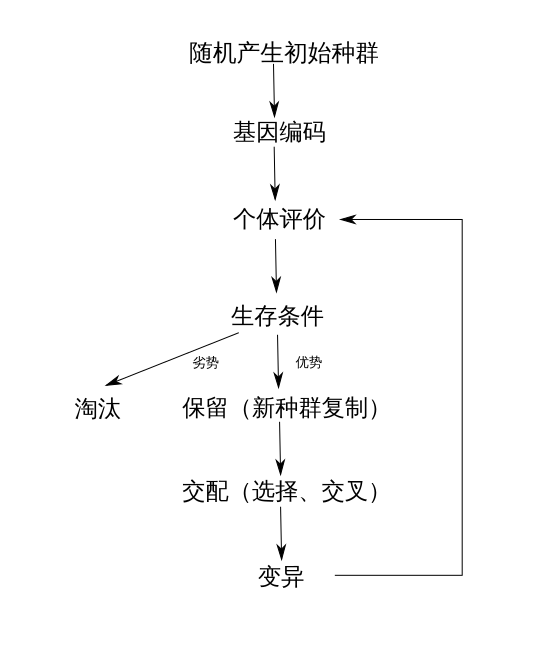
\includegraphics[width = 3in]{fig/遗传算法.png}
        \caption{遗传算法流程图}
        \label{fig1}
    \end{figure}
    \subsection{初始化}
        利用随机数产生一大小的样本空间,在这个样本空间中,不同的样本个体可能有截然不同的参数特性,它的多样性也保证了有足够的数据丰度以供自然选择。
    \subsection{编码}
        编码部分是多数遗传算法的接入部分,也是应用算法至关重要的一个部分。通过一定规则的编码,将外部信息转换成可以用于训练的二进制信息。编码方式的选择在很大程度上决定了遗传算法的可行性、适应性以及计算精度。
    \subsection{个体评价}
        通过将个体基因内容解码,再与既定优化趋势进行比较。与既定优化趋势相符合的为优势性状,反之为劣势性状,并且由目标偏离程度来计算得分。
    \subsection{生存条件}
        经过个体评价后,根据得分来筛除掉一部分个体,这种筛除可以是划线式的硬性筛除,也可以根据概率来筛除,比如转轮筛选法等。当然也可以二者结合,确定一个硬性红线,然后再做二次筛除,在保留一定数据丰度的同时提高算法效率,也可以结合神经网络做多路径筛选。
    \subsection{交配}
        剩下的个体在经过生存条件筛选后得以保留,获得了交配的权利,其中优势性状越多的个体获得交配的概率也就相对越高,优势性状得以传承。且交配过程中不同个体的染色体可以互换,产生新的性状。
    \subsection{变异}
        除了正常交换以外,还可能发生染色体变异$^{fig\ \ref{fig2}}$和基因突变现象。 
        \begin{figure}[htbp]
            \centering
            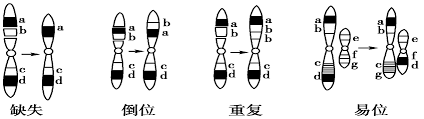
\includegraphics[width = 3in]{fig/染色体变异.png}
            \caption{染色体变异}
            \label{fig2}
        \end{figure}
    
        由生物学原理可知,基因经过交换可以产生新的基因型,但是无法产生新的基因,因此种群多样性受限。为了解决这一问题,我们采用加入一些随机数的方式来模拟小概率基因突变。这样做也是为了增加数据丰度,提供更多可能性。在变异完成之后新的种群重新进行自然选择的循环,直至预定目标。

\section{遗传算法优化电路参数}
    \subsection{编码}
        \begin{table}[htbp]
            \centering
            \begin{tabular}{|l|}
                \hline
                ... \\
                MPM5 ... W=100u L=.2u M=35 \\
                MPM6 ... W=4u L=1u M=1 \\
                MPM0 ... W=18u L=1u M=1 \\
                MPM2 ... W=4u L=1u M=1 \\
                MPM1 ... W=4u L=1u M=1 \\
                MNM1 ... W=2u L=7u M=1 \\
                MNM0 ... W=2u L=7u M=1 \\
                MNM3 ... W=6u L=2u M=1 \\
                MNM2 ... W=3u L=2.5u M=1 \\
                MPM4 ... W=20u L=1u M=1 \\
                MPM3 ... W=5u L=1u M=1 \\
                .END \\
                \hline
            \end{tabular}
            \caption{网表文件示意图}
            \label{table1}
        \end{table}
        在芯片设计中主要影响电路性能的参数就是各个 MOS 管的宽和长,以及它们之间的比例,因此编码也从这两个参数入手。考虑到二进制转换时候小数部分的精度问题,在这里需要做一些处理,比如先将所有数据都预先做倍乘处理,相当于将小数点的移位,等解码的时候再除回来。如果在其他模型中的参数为符号数,则可以引入补码机制来解决这一问题。考虑到数据处理上的方便,目前人为限定编码结果为固定长度,不足位则用0补充。
        
        在确定二进制转换方法之后,将每一个 MOS 管的宽和长作为一个小组进行编码,单个个体携带一整套编码,也即包含了电路中所有 MOS 管的信息,具体个体的编码长度由下计算: \\
        $$length = (W + L) * n$$
        
        W 和 L 分别代表编码宽度和长度所需二进制数的个数,n 代表初始网表中MOS管的数量,这一值由正则表达式格式化处理网表文件$^{table\ \ref{table1}}$后可得(详见FILEIO.read)。按照这种样式一共随机生成五百个(粗略数)个体作为初始种群。

        \begin{figure}[htbp]
            \centering
            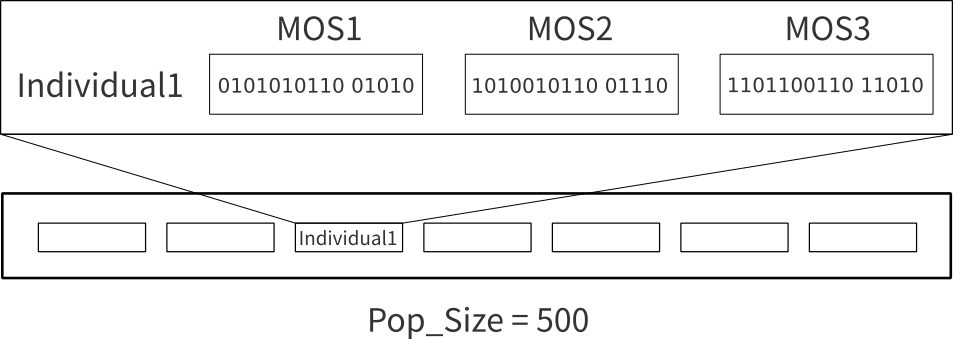
\includegraphics[width= 3in]{fig/encoding_black.png}
            \caption{编码}
            \label{fig3}
        \end{figure}
    \subsection{个体评价}
        针对不同的设计环境个体评价的方式也会不同,在本文中大体上来说有两个方向:变化趋势和指标权重。
        
        \textbf{变化趋势: }需要同历史数据进行比较判断某个指标变化的趋势,如果与目标趋势相同则加分,与目标趋势相悖则减分。 \\
        
        \textbf{指标权重: },也就是每个指标对于整体分数的影响,比如我需要设计一个运放,那么电压增益这一指标就可以适当提高权重。评价配置文件示例如下$^{table\ \ref{table2}}$,从左至右依次为指标名称、权重、目标趋势。
        
        \begin{table}[htbp]
            \centering
            \begin{tabular}{ccc}
                \toprule
                indicator & weight & trend \\
                \midrule
                A & 0.25 & + \\
                B & 0.63 & - \\
                C & 0.33 & + \\
                \bottomrule
            \end{tabular}
            \caption{评价标准示例}
            \label{table2}
        \end{table}
    
        考虑到配置文件容错性,一方面需要做查重处理,另外一方面就是要考虑到根据网表文件输出的分析结果来对应相应的指标评价标准,因此这里的权重设置为相对权重,评分方式也需要加入一定的自适应性。这里以从网表文件匹配到指标 A、C 为例,简单处理如下:\\
        $$Relative weight\ A = \pm \frac{A}{A+C}*Basic\ points$$ \\
        $$Relative weight\ C = \pm \frac{C}{A+C}*Basic\ points$$ \\
        由上得出 A、C 的绝对权重,最后个体得分采用加权平均计算。 \\
        $$\sum_{i=0}^{n} Indicator(i) * Weight(i)$$ 
        
    \subsection{生存条件}
        
\section{仿真和实验结果}

\end{document}

\begin{document}

\end{document} 